\documentclass[12pt,letterpaper]{article}

% Packages
\usepackage[utf8]{inputenc}
\usepackage[margin=1in]{geometry}
\usepackage{graphicx}
\usepackage{float}
\usepackage{hyperref}
\usepackage{enumitem}
\usepackage{titlesec}
\usepackage{fancyhdr}
\usepackage{tocloft}

% Header and footer
\pagestyle{fancy}
\fancyhf{}
\rhead{PlanInk User Manual v1.0.0}
\lhead{}
\cfoot{\thepage}

% Hyperlink settings
\hypersetup{
    colorlinks=true,
    linkcolor=blue,
    urlcolor=blue,
    citecolor=blue
}

% Title formatting
\titleformat{\section}
  {\normalfont\Large\bfseries}{\thesection}{1em}{}
\titleformat{\subsection}
  {\normalfont\large\bfseries}{\thesubsection}{1em}{}
\titleformat{\subsubsection}
  {\normalfont\normalsize\bfseries}{\thesubsubsection}{1em}{}

\begin{document}

% Title page
\begin{titlepage}
    \centering
    \vspace*{2cm}
    
    {\Huge\bfseries User Manual\par}
    \vspace{0.5cm}
    {\LARGE PlanInk 1.0.0\par}
    \vspace{2cm}
    
    {\Large Braden Dougherty\par}
    {\Large Lucas Landrus\par}
    {\Large Christopher Nguyen\par}
    {\Large Abdullah Orynbassar\par}
    \vspace{1cm}
    {\large Group 5\par}
    
    \vfill
    
    {\large December 1, 2025\par}
\end{titlepage}

% Table of contents
\tableofcontents
\newpage

% Main content
\section{Introduction}

\begin{center}\textbf{PlanInk can be found at \url{https://turing.cs.olemiss.edu:3005}}
\end{center}

\noindent Note: Requires web browser to have relaxed certificate validation protocol, such as Firefox or Safari


\subsection{Purpose}

The object of this user manual is to provide clients with the tools and knowledge necessary to utilize our system. Our current system is built for the University of Mississippi Engineering school, with scalability expected in later releases. Included will be notes for our different user types including engineering students, academic advisors, faculty, as well as development notes. The user will understand how to create and login to their account, and be able to use the features available to them, with detailed sections for each user role.

\subsection{Overview}

Our system is aimed at helping students, advisors, and faculty plan for future semesters. Students often feel overwhelmed and confused when scheduling classes for later semesters, while advisors can struggle to help students who may not know what their options and requirements are. Below are capabilities for each user role:\\\\
\textbf{Students:}
\begin{itemize}
    \item Can view current, advisor approved schedule
    \item Can view completed courses, and courses still left to take
    \item Can view further information about courses for clarity (Prerequisites, credits, description, etc)
    \item Can build a future schedule plan with an easy interface, save, and submit to advisor for review
\end{itemize}

\noindent \textbf{Advisors:}
\begin{itemize}
    \item Can see list of all students assigned to them, with ability to filter and search for individuals
    \item Ability to filter for students with schedules to review
    \item Further ability to accept or reject proposed schedules
    \item Can view an individual student's completed courses
    \item Can send messages to individual students to provide notes and guidance
    \item Can view change log of programs
\end{itemize}

\noindent \textbf{Faculty:}
\begin{itemize}
    \item Can view available majors
    \item Can update requirements for specific majors
    \item Can update individual courses
    \item Can view change log of programs
\end{itemize}

\subsection{System Requirements}

\begin{itemize}
    \item User must have internet access
    \item User must use a web browser capable of permitting user-initiated exceptions for TLS/SSL certificate validation failures. (e.g. Firefox)
\end{itemize}

\subsection{Version 1.0.0 Release}

This 1.0.0 release is geared towards the Computer science branch of the school of Engineering. With that being said, the currently supported majors include BSCS (Bachelor of Computer Science) and BSDS (Bachelor of Data Science). Our system is designed such that scalability is in the immediate future, and will be able to support a wider range of majors.

\section{Creating Accounts}

\subsection{Creating An Account}

When visiting the website, the login page is set up as shown below. To begin creating an account, select the ``signup'' button. After this, a signup page will appear as shown.

\begin{figure}[htb]
    \centering
    \begin{minipage}[b]{0.45\textwidth}
        \centering
        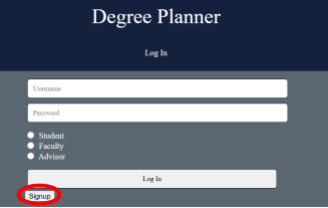
\includegraphics[width=1\linewidth]{images/image12.png}
    \end{minipage}\hfill
    \begin{minipage}[b]{0.45\textwidth}
        \centering
        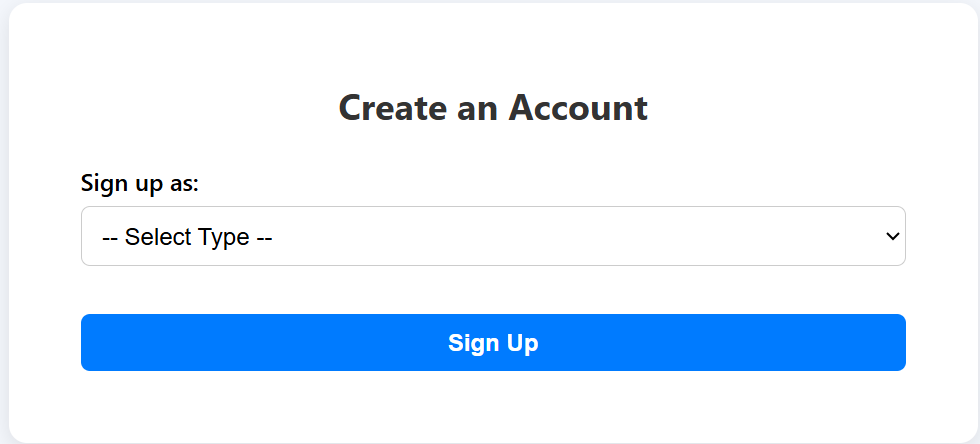
\includegraphics[width=1\linewidth]{images/image13.png}
    \end{minipage}
\end{figure}

\subsubsection{Creating Student Account}

\newpage

To begin, select ``Student'' in the dropdown menu.
\begin{figure}[htb]
    \centering
    \begin{minipage}[b]{0.45\textwidth}
        \centering
        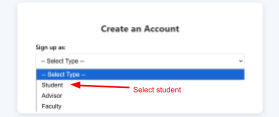
\includegraphics[width=1\linewidth]{images/image2.png}
    \end{minipage}\hfill
    \begin{minipage}[b]{0.45\textwidth}
        \centering
        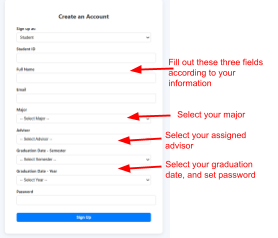
\includegraphics[width=1\linewidth]{images/image10.png}
    \end{minipage}
\end{figure}

After submitting the form, you will be redirected to the login page.



\subsubsection{Creating Advisor Account}

To begin, select advisor from the drop down menu.
\begin{figure}[htb]
    \centering
    \begin{minipage}[b]{0.45\textwidth}
        \centering
        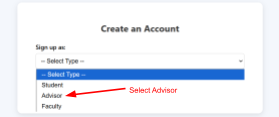
\includegraphics[width=1\linewidth]{images/image11.png}
    \end{minipage}\hfill
    \begin{minipage}[b]{0.45\textwidth}
        \centering
        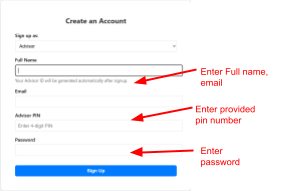
\includegraphics[width=1\linewidth]{images/image4.png}
    \end{minipage}
\end{figure}

To prevent bad actors from creating advisors and faculty users, sample pins were created. The advisor pin is \textbf{1111}. After filling out and submitting the form, the user will be redirected to the login page.

To reset the pin, contact our team. (Contact available at end)

\newpage

\subsubsection{Creating Faculty Account}

To begin, select faculty from the dropdown menu.
\begin{figure}[htb]
    \centering
    \begin{minipage}[b]{0.45\textwidth}
        \centering
        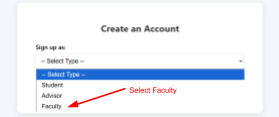
\includegraphics[width=1\linewidth]{images/image6.png}
    \end{minipage}\hfill
    \begin{minipage}[b]{0.45\textwidth}
        \centering
        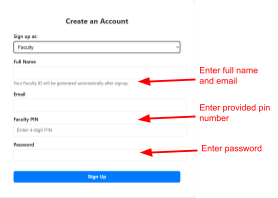
\includegraphics[width=1\linewidth]{images/image3.png}
    \end{minipage}
\end{figure}

To prevent bad actors from creating advisors and faculty users, sample pins were created. The faculty pin is \textbf{2222}. After filling out and submitting the form, the user will be redirected to the login page.

To reset the pin, contact our team. (Contact available at end)

\subsection{Logging In}

Follow the shown steps to log in to your respective user portal.

\begin{figure}[htb]
      \centering
      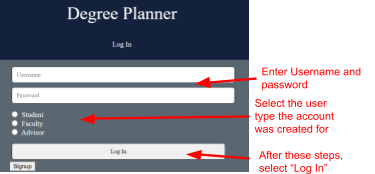
\includegraphics[width=1\linewidth]{images/image9.png}
\end{figure}


\section{Students}

\subsection{Student Portal}

The student portal consists of the following sections:

\begin{enumerate}
    \item In this section, the student can see their anticipated graduation date, as well as a logout button to end their session.
    
    \item In this section, the student can access another page (Full functionality explained in sections 3.1.1--3.1.4)
    \begin{itemize}
        \item \textbf{Progress} - Student can view completed courses, as well as completed hours out of required total hours for their major
        \item \textbf{Sandbox} - Interactive user interface to build future schedules that can be submitted to advisor
        \item \textbf{Classes} - Student can view full list of relevant courses to their major
        \item \textbf{Approved Schedule} - Students can view their advisor-approved schedule
    \end{itemize}
    
    \item In this section, comments that the advisor has sent to the student are available to see
    \begin{itemize}
        \item These comments can either be schedule rejection comments (The submitted schedule needs to be tweaked), or general comments.
        \item The green ``Mark as Resolved'' button clears the comment from the student portal
    \end{itemize}
    \begin{figure}[htb]
      \centering
      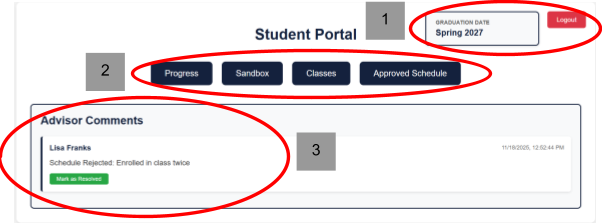
\includegraphics[width=1\linewidth]{images/image7.png}
    \end{figure}
\end{enumerate}

\subsubsection{Student Progress}

To access this page, begin by selecting the ``Progress'' button in the student portal.
    \begin{figure}[htb]
    \centering
      \begin{minipage}[b]{0.55\textwidth}
        \centering
        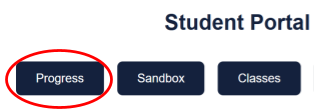
\includegraphics[width=1\linewidth]{images/image1.png}
      \end{minipage}
    \end{figure}

\begin{enumerate}

    \item This ``Back to Student Portal'' button returns the student to the student portal.
    \item Included logout button to end session
    \item This section displays the total number of hours completed for the student, as well as the number of hours needed to complete their degree.
    \item This section displays the courses that have been completed for the student.
    \begin{figure}[htb]
        \centering
        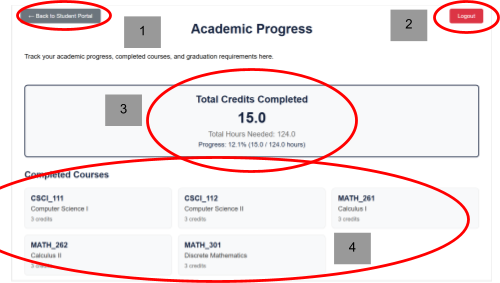
\includegraphics[width=1\linewidth]{images/image5.png}
    \end{figure}
\end{enumerate}

\subsubsection{Student Sandbox}

To begin, select the ``Sandbox'' button in the student portal.
    \begin{figure}[htb]
    \centering
      \begin{minipage}[b]{0.55\textwidth}
        \centering
        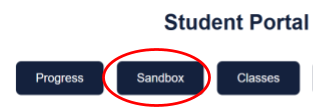
\includegraphics[width=1\linewidth]{images/image8.png}
      \end{minipage}
    \end{figure}

\begin{enumerate}

    \item This ``Back to Student Portal'' button returns the student to the student portal.

    \begin{figure}[H]
        \centering
        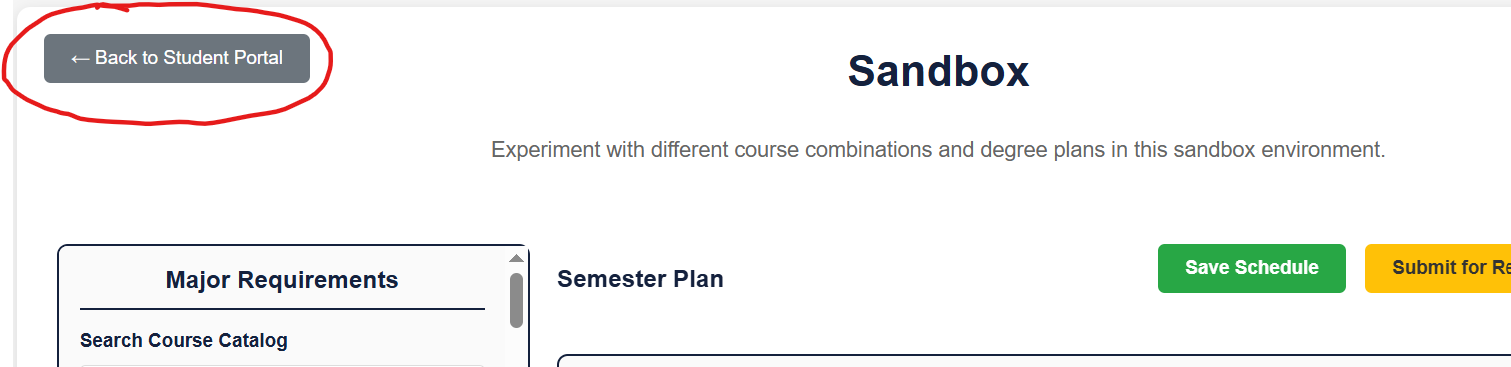
\includegraphics[width=1\linewidth]{images/image#.png}
    \end{figure}
\end{enumerate}
 
    \subsubsection{Sandbox — Building a Schedule}

    The Sandbox is the primary tool students use to construct future schedules. It provides a drag-and-drop interface where courses are represented as cards that can be placed into term columns. The sandbox preserves prerequisite warnings and highlights courses that conflict by time or requirement.

    Key features:
    \begin{itemize}
        \item Drag-and-drop course cards between terms and remove courses with the \textbf{Remove} action.
        \item Real-time prerequisite checking and visual indicators for unmet requirements.
        \item Credit hour totals per term and cumulative totals for planned terms.
        \item Save drafts locally to continue later, or submit to your advisor for review.
    \end{itemize}

    \begin{figure}[H]
        \centering
        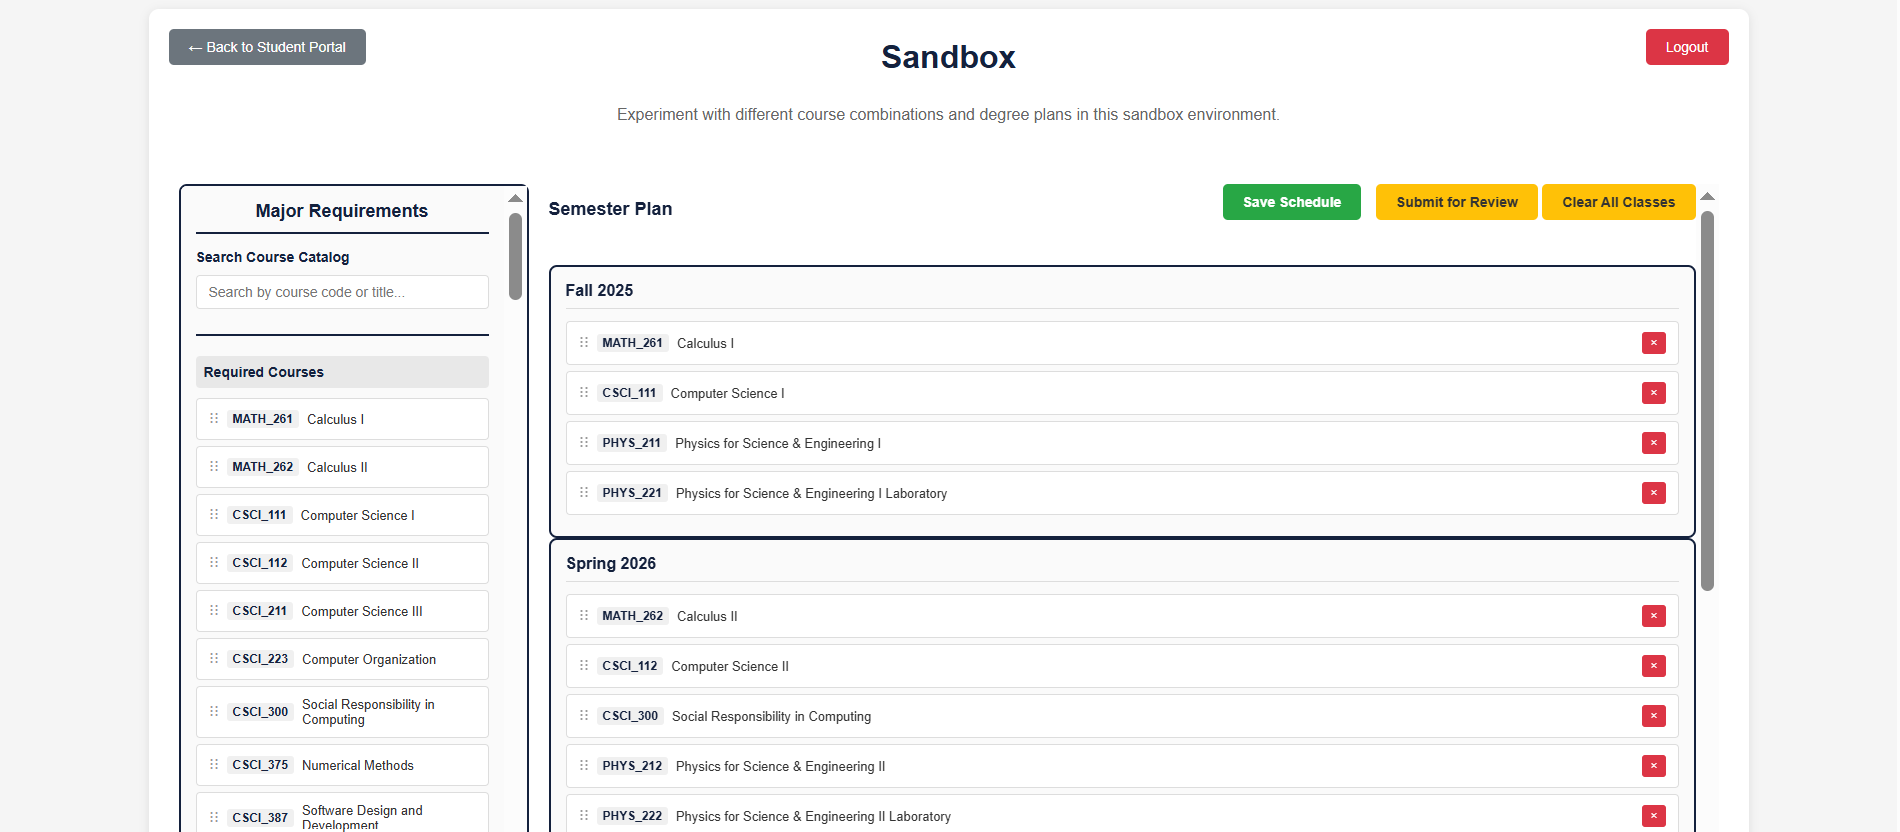
\includegraphics[width=1\linewidth]{images/student_sandbox_extended.png}
    \end{figure}

    \subsubsection{Saving and Submitting a Sandbox}

    Students can save a sandbox draft at any time using the \textbf{Save} button. To request advisor review, use the \textbf{Submit to Advisor} button which creates a pending submission entry visible to both the student and assigned advisor.

    When submitting:
    \begin{itemize}
        \item Add an optional message to the advisor explaining special requests or constraints.
        \item The submission is time-stamped and appears in the advisor's \textit{Schedules to Review} list.
        \item If the advisor requests changes, the submission returns to the student's sandbox with advisor comments attached.
    \end{itemize}

    \begin{figure}[H]
        \centering
        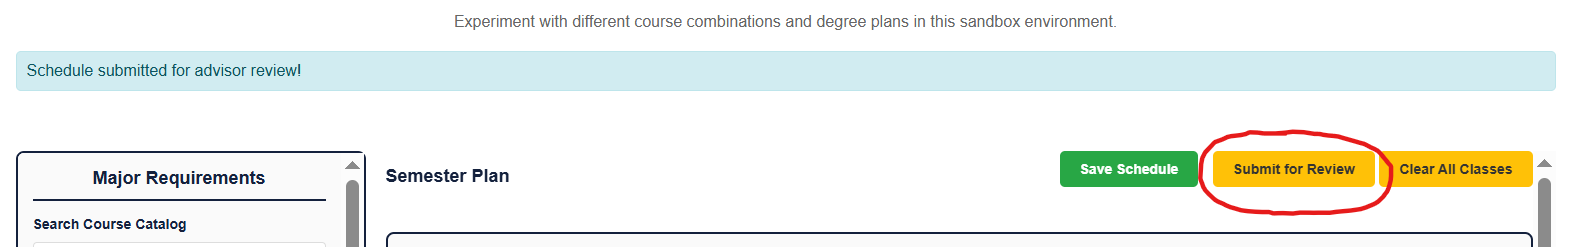
\includegraphics[width=0.9\linewidth]{images/student_submit_placeholder.png}
    \end{figure}

    \subsubsection{Classes}

    The \textbf{Classes} view lists all courses relevant to the student's major and minor (where applicable). Students can search, filter by subject or level, and open detail views for each course to view prerequisites, credits, and descriptions.

    Functions available in the Classes view:
    \begin{itemize}
        \item Search bar to find courses by name or code.
        \item Filters for subject area, elective vs required, and credit hours.
        \item Click a course to open an information panel with full description, prerequisites, and suggested terms.
        \item From the course panel, use \textbf{Add to Sandbox} to place the course into the current sandbox term.
    \end{itemize}

    \begin{figure}[H]
        \centering
        \begin{minipage}[b]{0.45\textwidth}
            \centering
             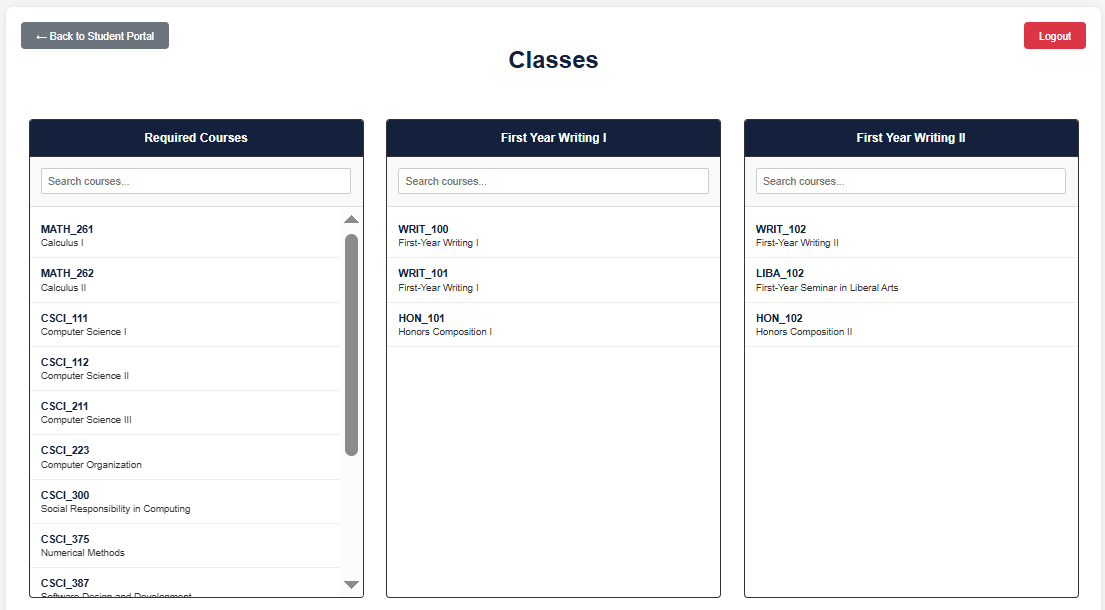
\includegraphics[width=1\linewidth]{images/student_classes_placeholder.png}
        \end{minipage}
        \begin{minipage}[b]{0.45\textwidth}
            \centering
            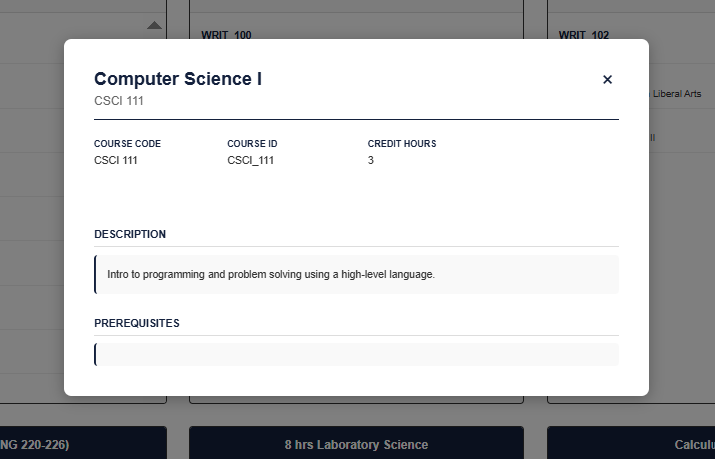
\includegraphics[width=1\linewidth]{images/student_classes_placeholder2.png}
        \end{minipage}\hfill
    \end{figure}

    \subsubsection{Approved Schedule}

    The \textbf{Approved Schedule} view shows the student's current advisor-approved course plan. Approved schedules are read-only for students; any further changes should be made in the Sandbox and re-submitted for approval.

    What to expect in the Approved Schedule:
    \begin{itemize}
        \item A semester-by-semester layout mirroring the sandbox but locked for editing.
        \item Approval metadata including approving advisor name and approval date.
        \item A \textbf{Request Change} button to notify the advisor if an approved schedule requires modification.
    \end{itemize}

    \begin{figure}[H]
        \centering
        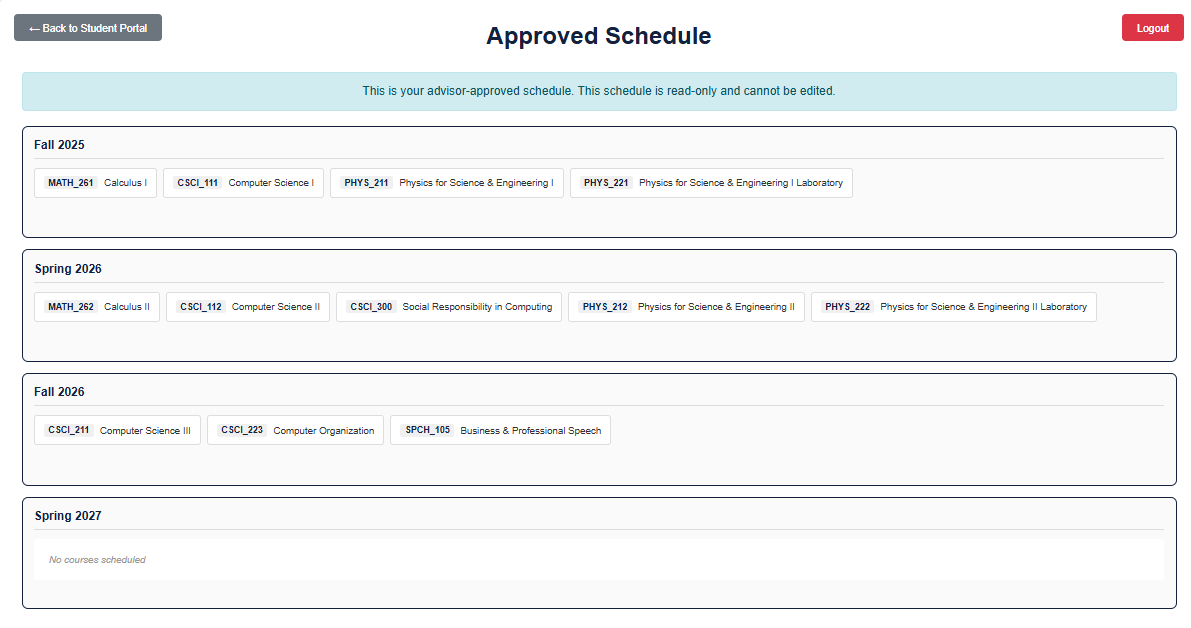
\includegraphics[width=1\linewidth]{images/approved_schedule_placeholder.png}
    \end{figure}

    \subsubsection{Notifications and Messages}

    Students receive notifications when advisors comment on a submission, when approvals are made, and when account-related events occur. Notifications appear in the student portal header and in the messages panel.

    \begin{itemize}
        \item Click a notification to navigate to the related sandbox or comment thread.
        \item Use the messages panel to send or reply to advisor communications; mark messages as resolved to clear them from the primary portal view.
    \end{itemize}

    \begin{figure}[H]
        \centering
        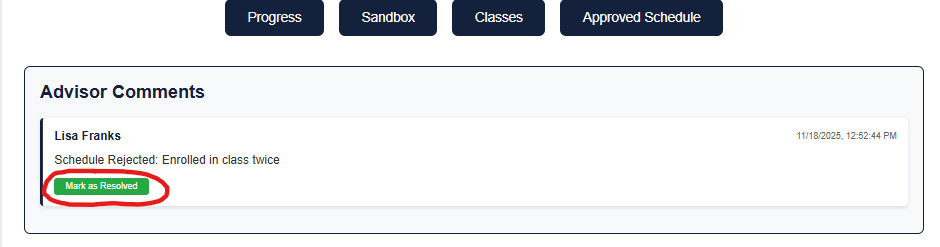
\includegraphics[width=1\linewidth]{images/student_notifications_placeholder.png}
    \end{figure}

    \newpage

\section{Advisors}

\subsection{Advisor Portal}

The advisor portal is designed to help academic advisors efficiently review and manage student schedules. Main features include a searchable student list, quick filters for schedules pending review, and direct message ability for student guidance.

\begin{enumerate}
    \item The header includes the advisor's name, a logout button, and a quick summary of schedules awaiting review.
    \item In the left navigation, advisors can access: \textbf{Students}, \textbf{Schedules to Review}, \textbf{Change Log}, and \textbf{Messages}.
    \item The central area displays the selected student's profile and submitted sandbox schedule for review.
    \item The right panel includes quick actions: approve, request changes, or send a message to the student.
\end{enumerate}

\begin{figure}[H]
    \centering
    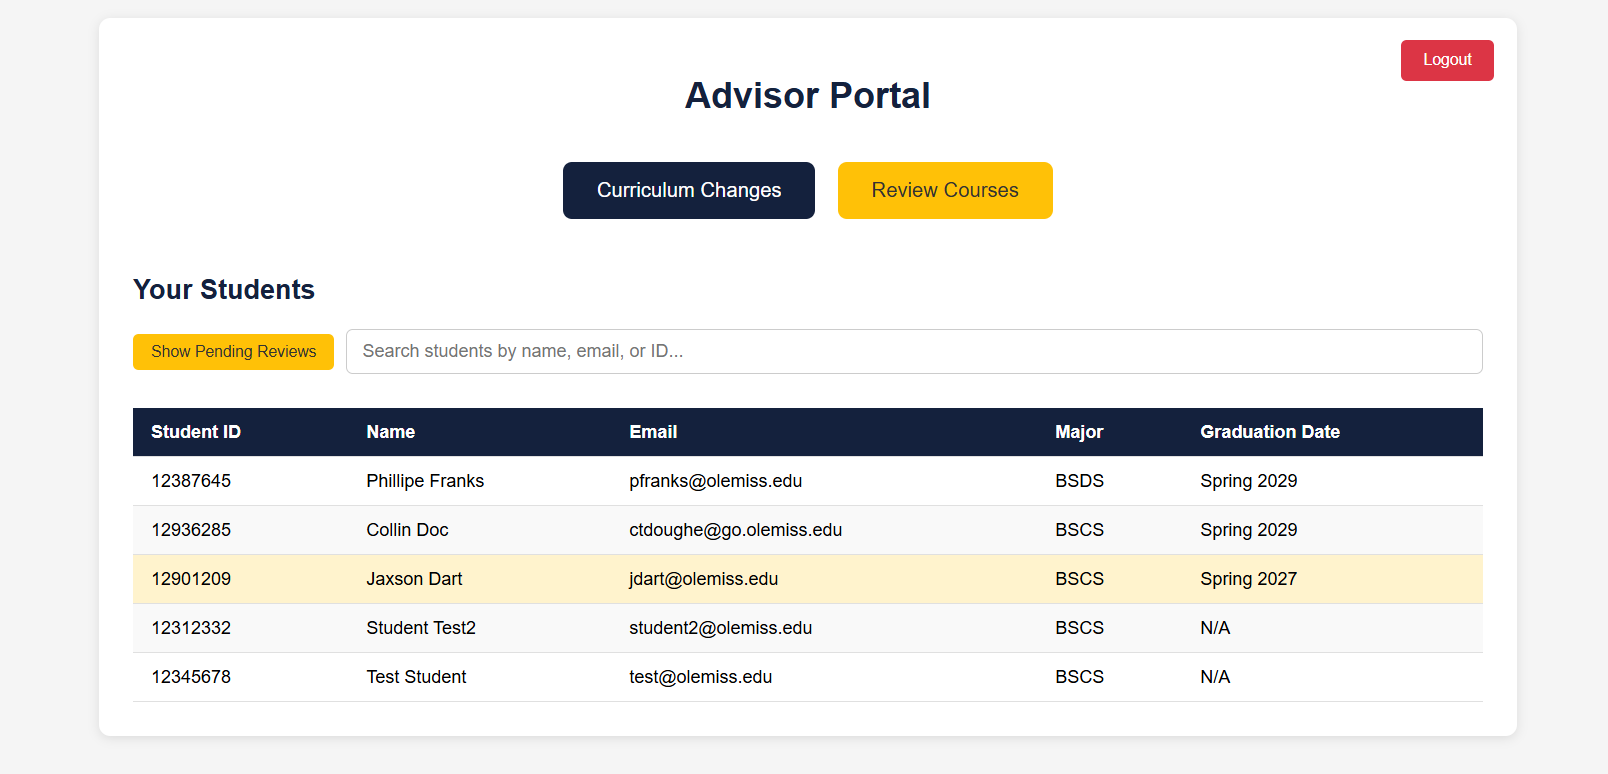
\includegraphics[width=1\linewidth]{images/advisor_portal.png}
\end{figure}

\subsection{Reviewing Student Schedules}

To review a student's proposed schedule:

\begin{enumerate}
    \item Select the student from the advisor's student list.
    \begin{figure}[H]
        \centering
        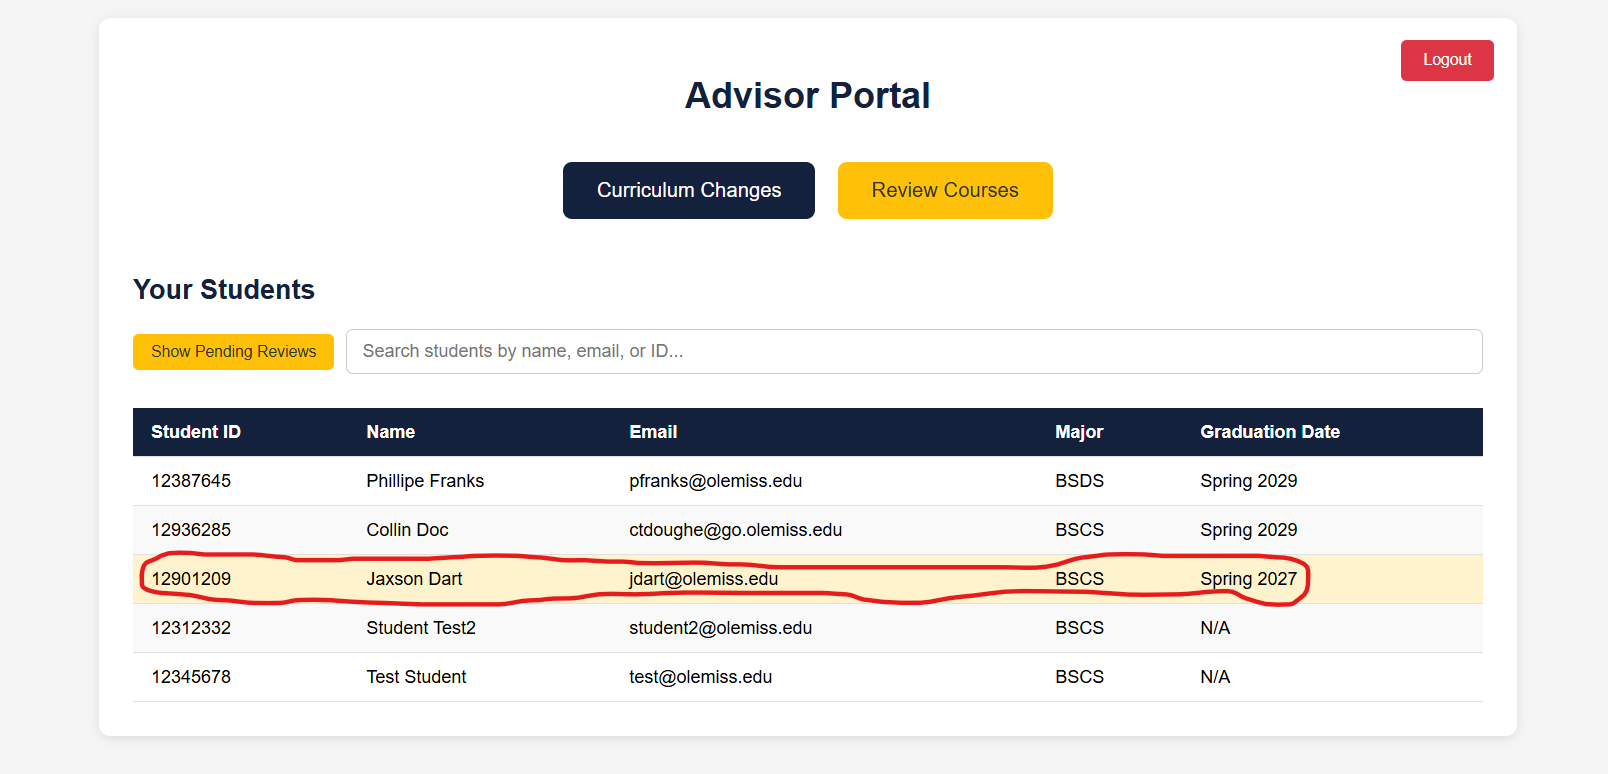
\includegraphics[width=1\linewidth]{images/studentSchedule1.png}
    \end{figure}
    \item Open the submitted schedule in the central view.
    \item Use the notes field to provide feedback; these comments will appear in the student's portal.
    \item Use the \textbf{Accept} button to approve the schedule, or \textbf{Request Changes} to send it back with notes.
\end{enumerate}

\begin{figure}[H]
    \centering
    \begin{minipage}[b]{0.45\textwidth}
        \centering
        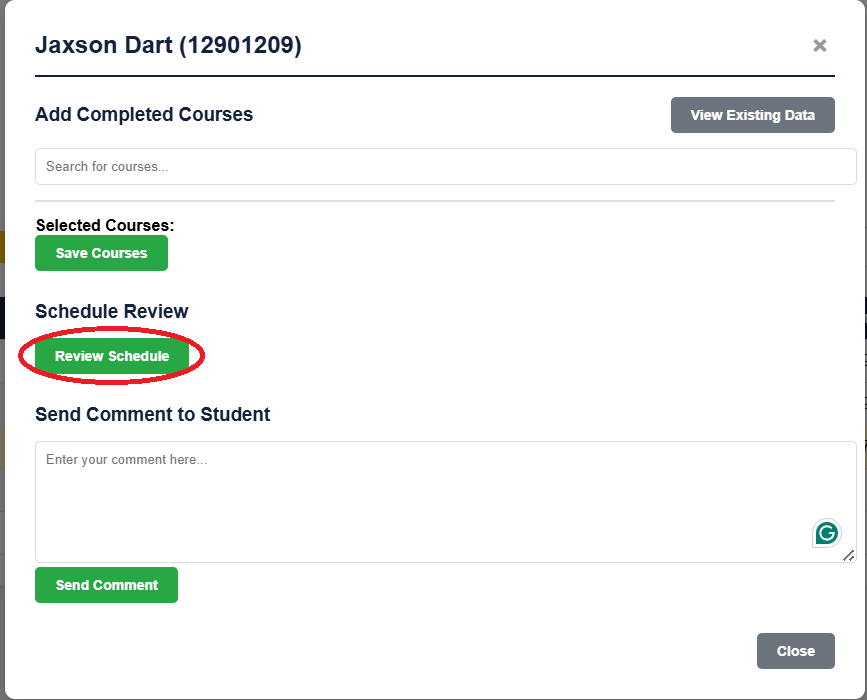
\includegraphics[width=1\linewidth]{images/studentSchedule2.png}
    \end{minipage}
    \begin{minipage}[b]{0.45\textwidth}
        \centering
        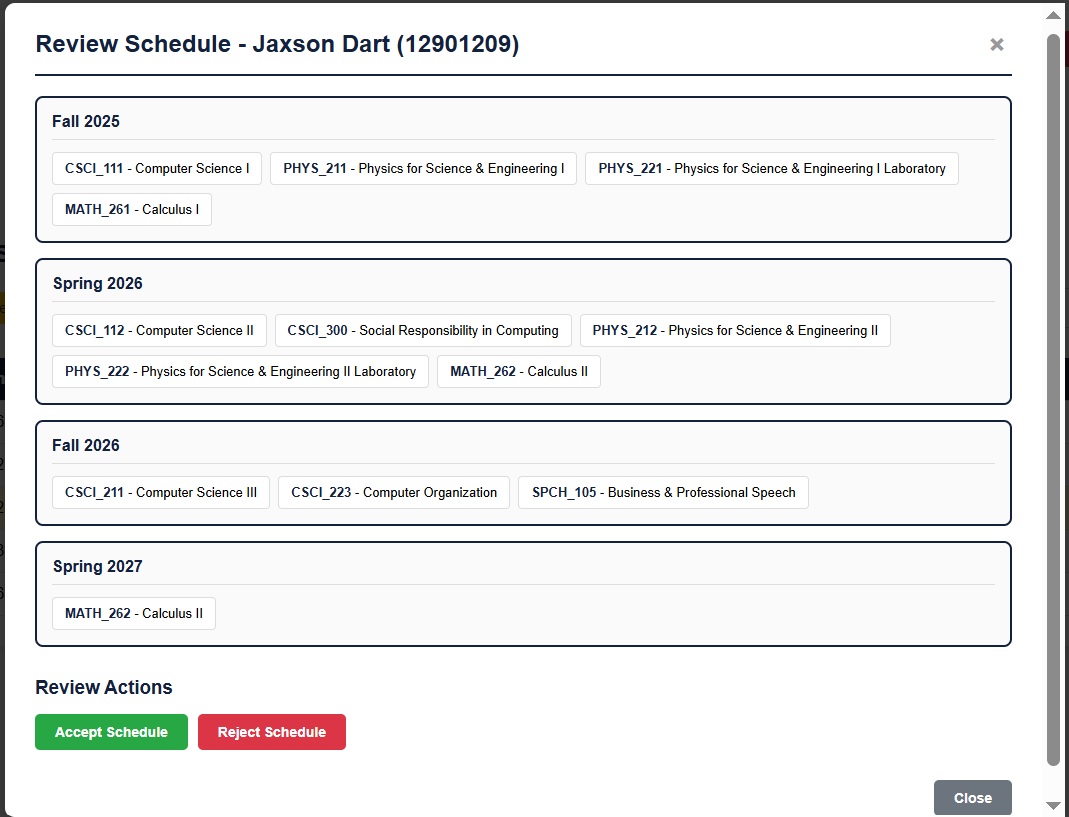
\includegraphics[width=1\linewidth]{images/studentSchedule3.png}
    \end{minipage}\hfill
\end{figure}

\subsection{Change Log}

Advisors can view a complete change log for programs and course requirement updates. The change log shows the timestamp, author, and description of each change.

\begin{figure}[H]
    \centering
    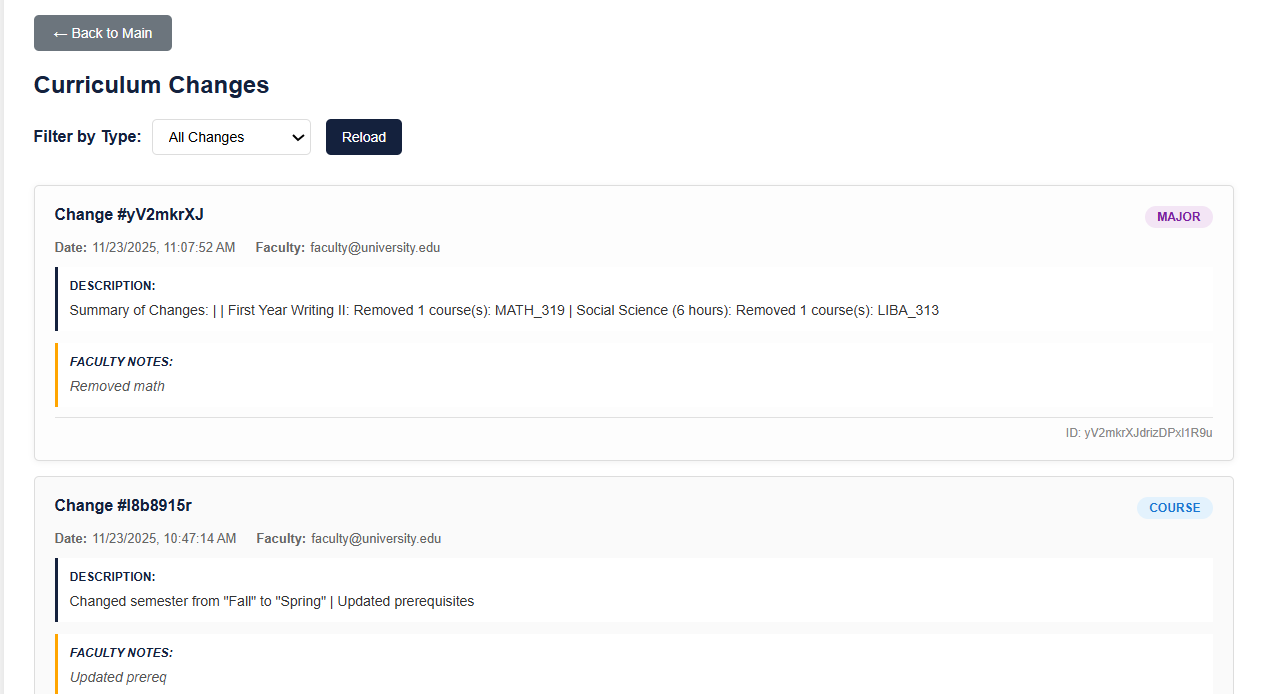
\includegraphics[width=1\linewidth]{images/change_log.png}
\end{figure}
\subsubsection{Advisor Dashboard}

\subsubsection{Student List and Filters}

The student list is the primary navigation for advisors to find and manage assigned students. Use the search bar, filters, and sorting to narrow the list.

Common controls and columns:
\begin{itemize}
    \item \textbf{Search:} Search by name, student ID, or email.
    \item \textbf{Filters:} Filter by major, academic standing, or schedules pending review.
    \item \textbf{Columns:} Name, Major, GPA (if available), Last Submission Date, Status, and Quick Actions.
    \item \textbf{Quick Actions:} View profile, open latest submission, or send a message.
\end{itemize}

\begin{figure}[H]
    \centering
    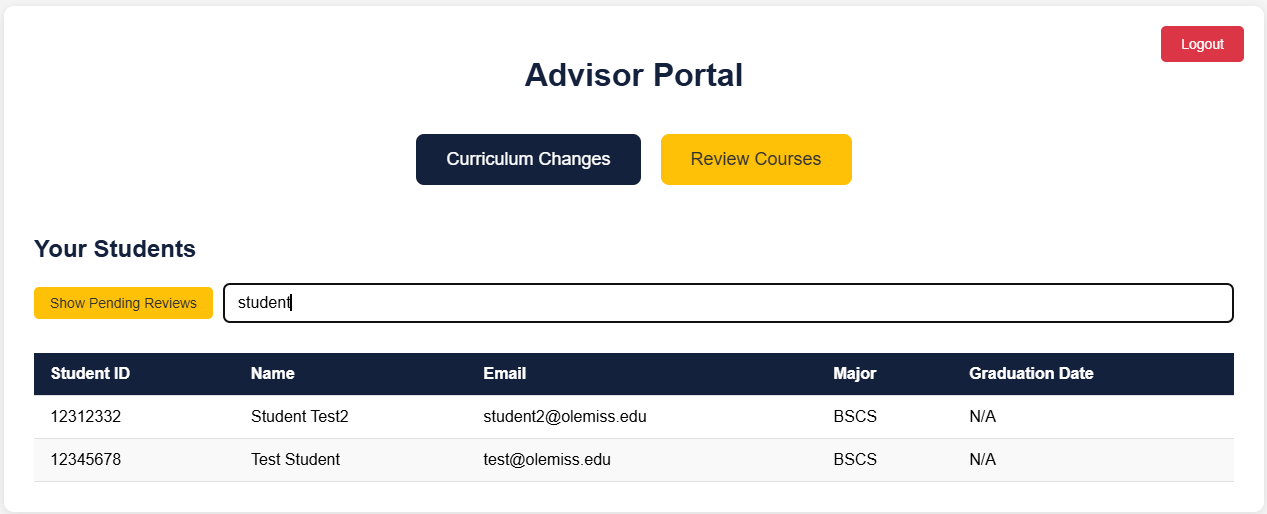
\includegraphics[width=1\linewidth]{images/advisor_student_list.png}
\end{figure}

\subsubsection{Review Dialog and Actions}

When opening a student's submission, advisors see a detailed review dialog containing the submitted schedule, course metadata, and any attached student notes.

Review flow:
\begin{enumerate}
    \item Inspect the submitted terms and courses in a read-only schedule pane.
    \item Use the comment field to add targeted feedback on courses or terms.
    \item Choose \textbf{Approve} to finalize the schedule or \textbf{Request Changes} to return it to the student with comments.
    \item Optionally attach recommended course substitutions or links to relevant resources.
\end{enumerate}

\begin{figure}[H]
    \centering
    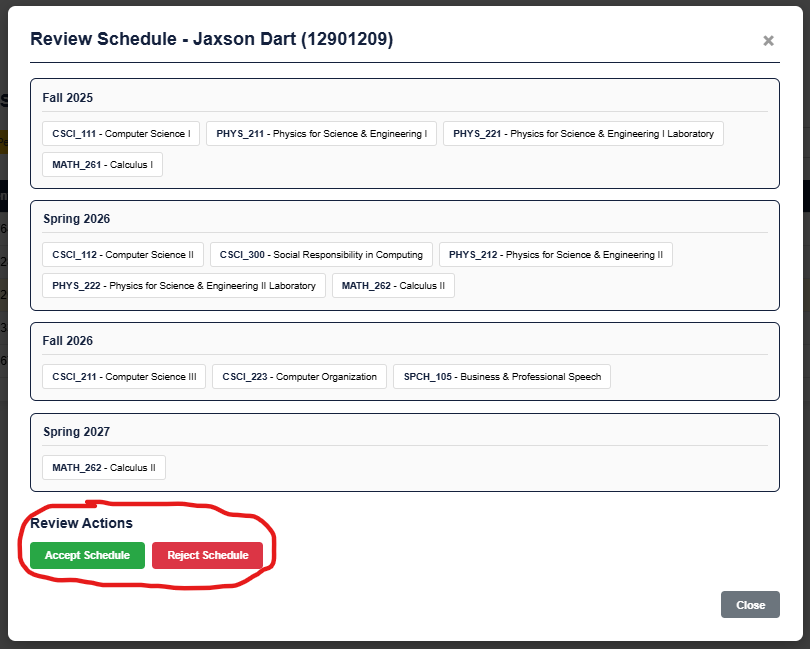
\includegraphics[width=1\linewidth]{images/advisor_review_dialog.png}
\end{figure}

\subsubsection{Messaging and Notes}

Advisors can send targeted messages to students either from the student list, profile view, or within a submission review. Messages are threaded and stored with reference to the related submission when applicable.

Messaging features:
\begin{itemize}
    \item Threaded view with timestamps and sender labels.
    \item Ability to attach links or references to program requirements and course pages.
    \item Mark messages as resolved to clear them from the advisor's primary dashboard.
\end{itemize}

\begin{figure}[H]
    \centering
    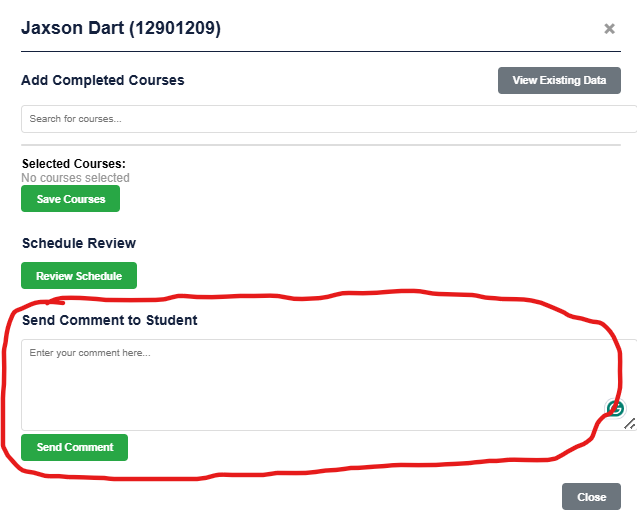
\includegraphics[width=0.8\linewidth]{images/advisor_message_thread.png}
\end{figure}

\subsubsection{Change Log Details and Auditing}

The change log provides a complete history of program and course requirement modifications. Advisors can filter the change log to show recent updates relevant to their students or export entries for review.

Change log capabilities:
\begin{itemize}
    \item Filter by date range, author, or program affected.
    \item View full diff of requirement changes where available.
    \item Export filtered results to CSV for departmental review.
\end{itemize}

\begin{figure}[H]
    \centering
    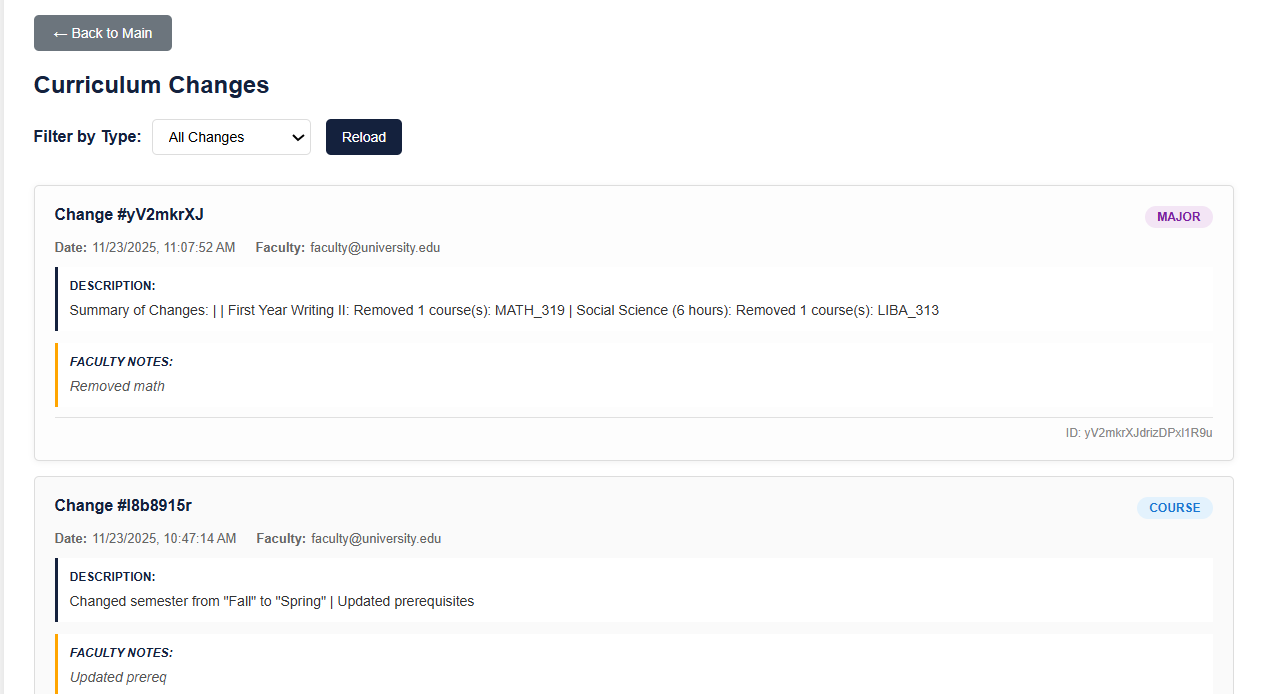
\includegraphics[width=1\linewidth]{images/change_log.png}
\end{figure}

\newpage

\section{Faculty}

\subsection{Faculty Portal}

Faculty users can view and update majors, course details, and program requirements. The portal provides safe edit capabilities and records every update in the change log.

\begin{enumerate}
    \item Faculty header: name, department, and logout button.
    \item Navigation: \textbf{Majors}, \textbf{Courses}, \textbf{Change Log}.
    \item Editing views include form fields for course description, credits, and prerequisites.
\end{enumerate}

\begin{figure}[H]
    \centering
    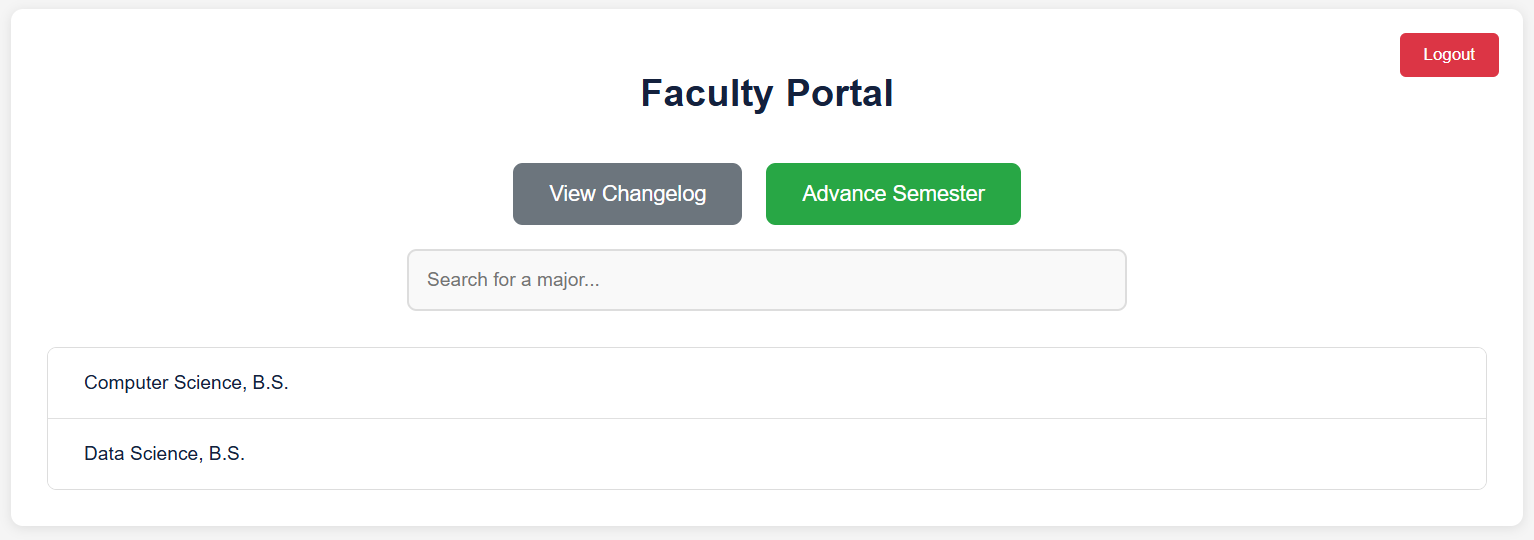
\includegraphics[width=1\linewidth]{images/faculty_portal.png}
\end{figure}

\subsection{Updating Requirements and Courses}

When editing a major or course:

\begin{enumerate}
    \item Select the major or course from the list.
    \item Edit the required fields and click \textbf{Save Changes}.
    \item All changes are recorded in the change log with the user's details and timestamp.
    \item Major-level edits can include adding/removing course requirements and adjusting credit totals.
\end{enumerate}

\begin{figure}[H]
    \centering
    \begin{minipage}[b]{0.45\textwidth}
        \centering
        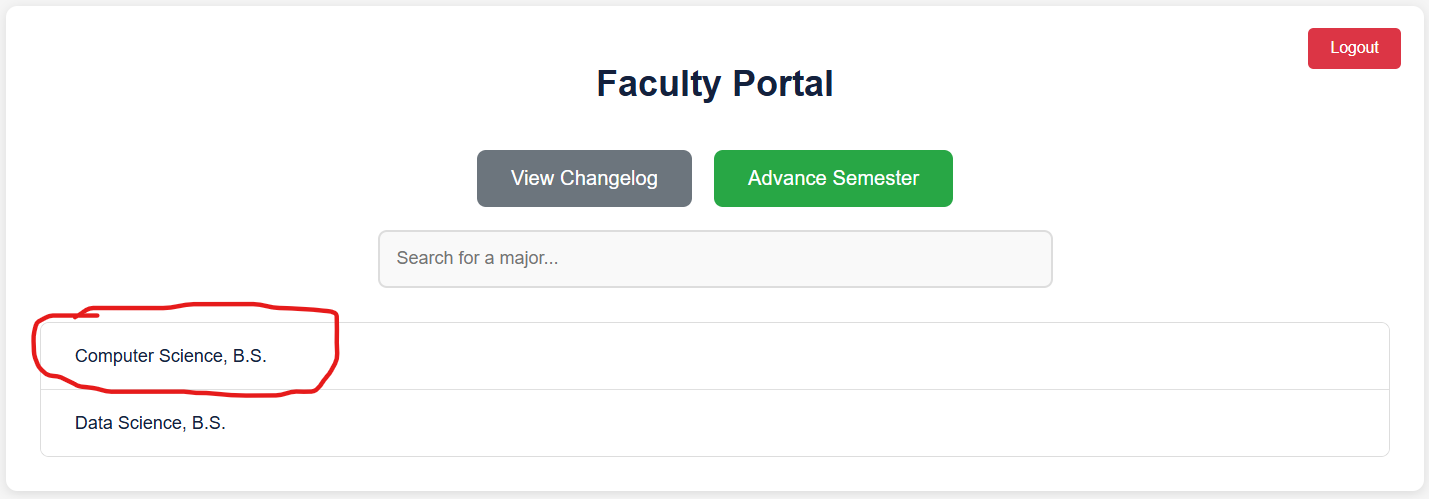
\includegraphics[width=1\linewidth]{images/clickMajor.png}
    \end{minipage}
    \begin{minipage}[b]{0.45\textwidth}
        \centering
        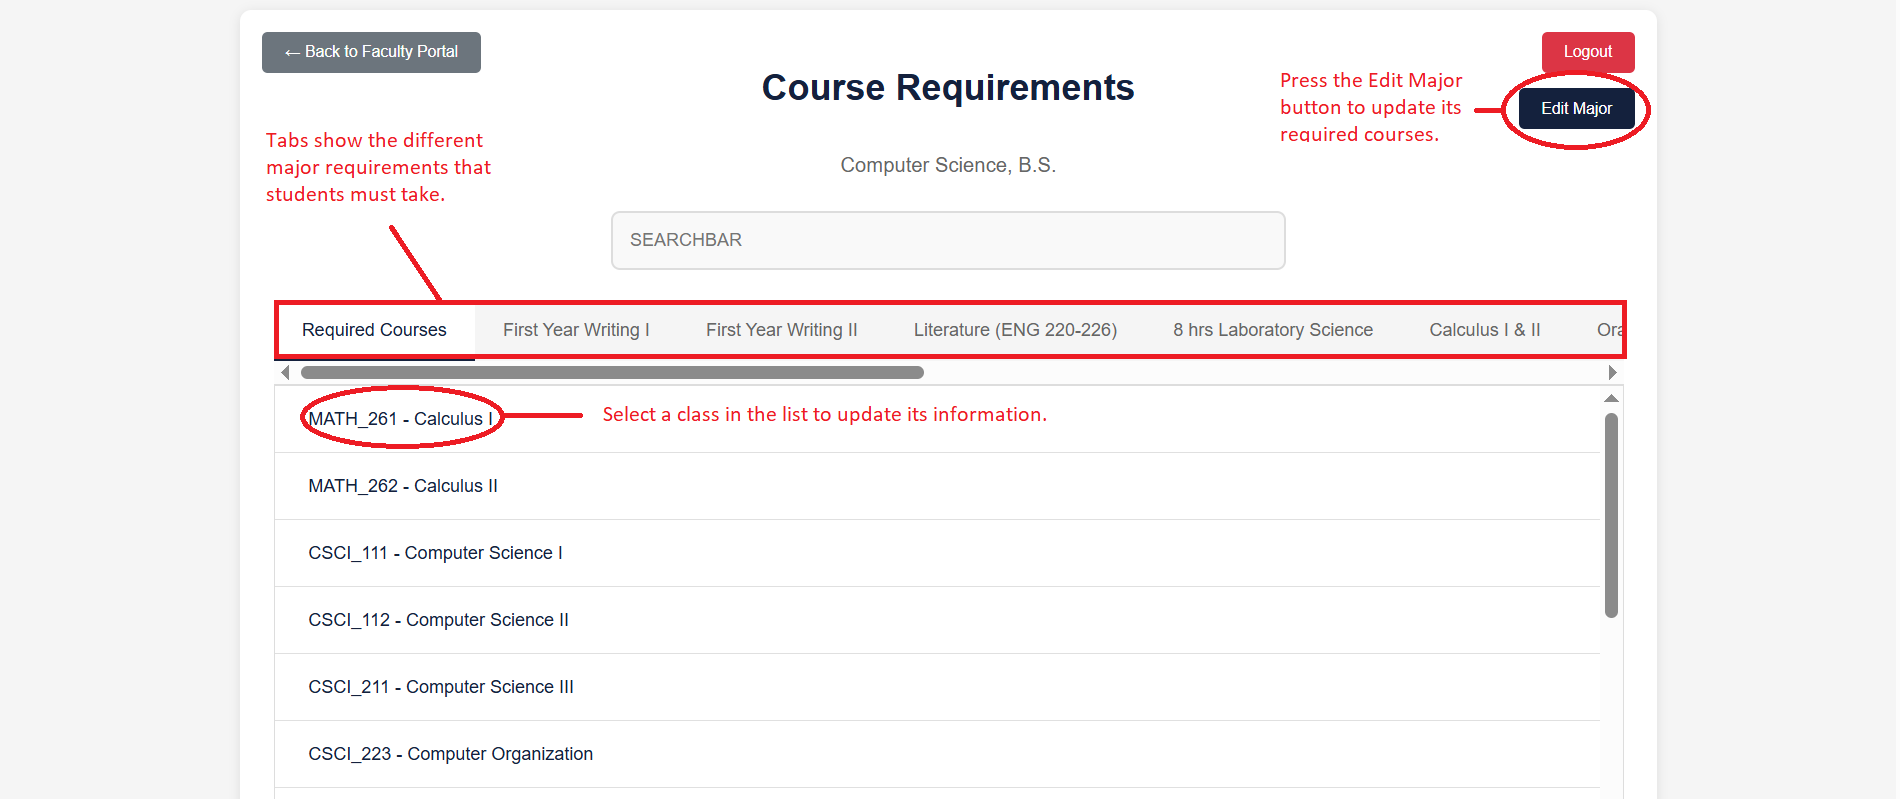
\includegraphics[width=1\linewidth]{images/courseReqs.png}
    \end{minipage}\hfill
\end{figure}

\begin{figure}[H]
    \centering
    \begin{minipage}[b]{0.45\textwidth}
        \centering
        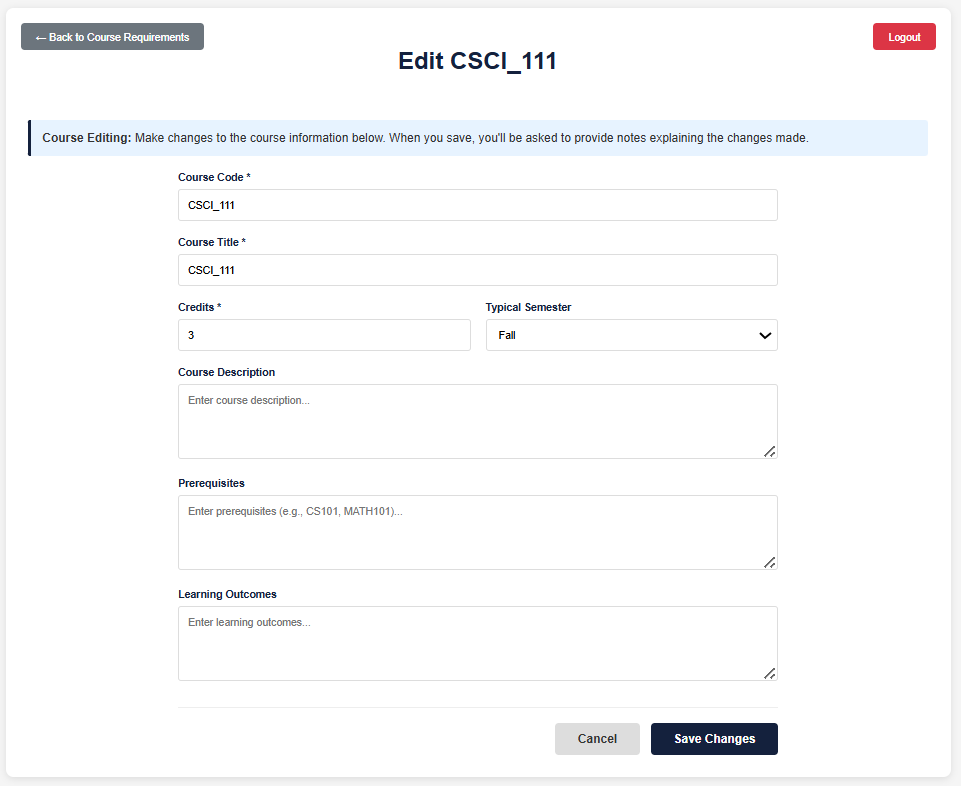
\includegraphics[width=1\linewidth]{images/editCourse.png}
    \end{minipage}
    \begin{minipage}[b]{0.45\textwidth}
        \centering
        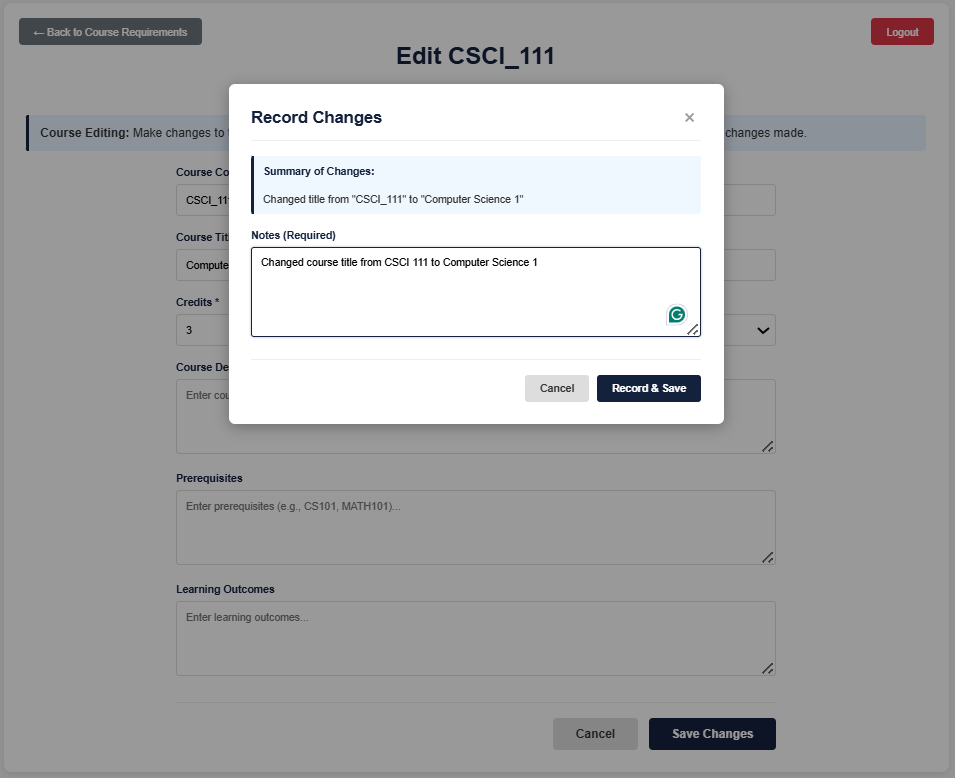
\includegraphics[width=1\linewidth]{images/editCourse2.png}
    \end{minipage}\hfill
\end{figure}
\subsubsection{Faculty Dashboard}

The Faculty Dashboard gives a concise view of department-level tasks and recent program activity. Faculty will see pending change requests, recently edited courses, and high-level enrollment notes.

Dashboard elements:
\begin{itemize}
    \item \textbf{Pending Change Requests:} Requests from faculty or admin to modify requirements or course data.
    \item \textbf{Recent Edits:} Quick list of recently edited courses or majors with short descriptions.
    \item \textbf{Department Notices:} Announcements relevant to curriculum changes or deadlines.
\end{itemize}

\subsubsection{Majors Management}

Faculty can manage majors through a dedicated Majors view. This view lists all majors under the faculty's purview and allows navigation to edit requirement groups, elective buckets, and credit totals.

Majors view features:
\begin{itemize}
    \item \textbf{List of Majors:} Click to open details for a selected major.
    \item \textbf{Requirement Groups:} View and reorder requirement groups (core, electives, technical electives).
    \item \textbf{Credit Overview:} Summary of total credits required and credits allocated to each group.
\end{itemize}

\begin{figure}[H]
    \centering
    \begin{minipage}[b]{0.45\textwidth}
        \centering
        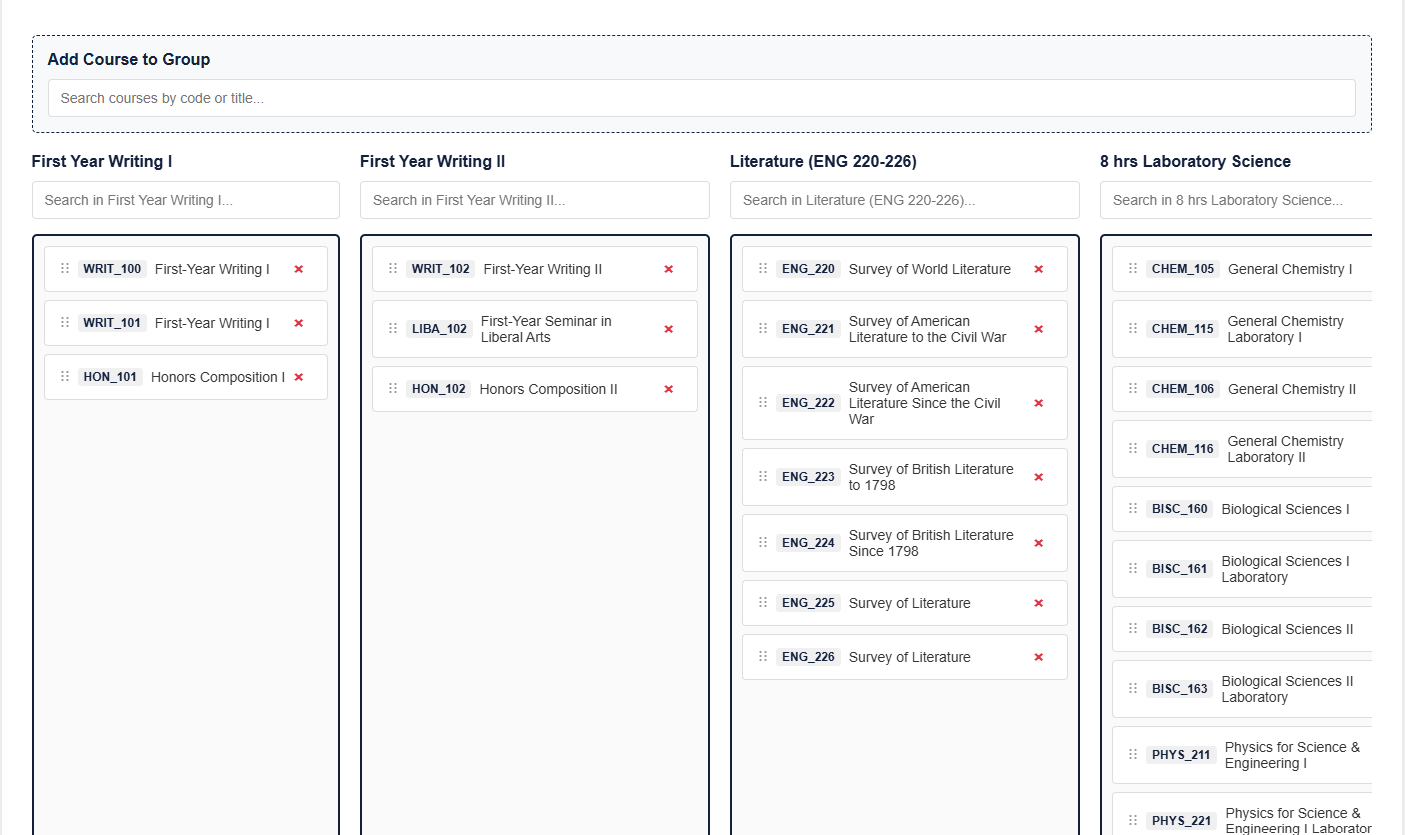
\includegraphics[width=1\linewidth]{images/editMajor.png}
    \end{minipage}
    \begin{minipage}[b]{0.45\textwidth}
        \centering
        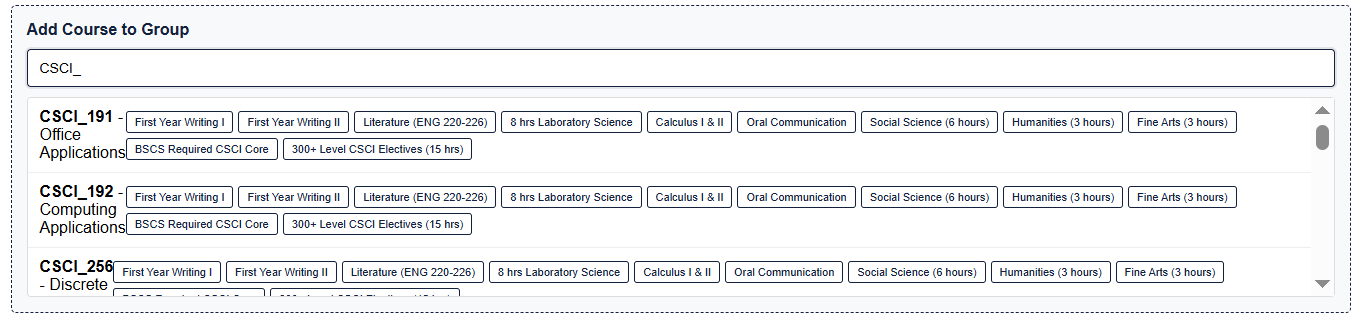
\includegraphics[width=1\linewidth]{images/editMajor2.png}
    \end{minipage}\hfill
\end{figure}

\subsubsection{Course Editor}

The Course Editor provides form-based editing for course properties including title, description, credits, prerequisites, and cross-listings. Edits are validated and previewed before saving.

Course editor capabilities:
\begin{itemize}
    \item Edit course title, description, and credit hours.
    \item Update prerequisites and corequisites with autocomplete for course codes.
    \item Add or remove cross-listed sections and note department ownership.
    \item Preview the course as it will appear to students prior to saving.
\end{itemize}


\subsubsection{Requirement Editor and Buckets}

Faculty can edit requirement buckets (e.g., Core, Electives, Technical) within a major. The editor supports adding/removing courses from buckets and specifying minimum/maximum credit constraints.

Requirement editor features:
\begin{itemize}
    \item Drag-and-drop interface to move courses into requirement buckets.
    \item Set bucket constraints such as minimum credit hours or required course counts.
    \item Mark substitutions or allowed course alternatives for flexibility in degree audits.
\end{itemize}

\subsubsection{Publishing Changes and Approvals}

Faculty edits may require departmental review before being published. The system tracks drafts and publishes changes after approvals, recording authorship and timestamps for auditing.

Publishing workflow:
\begin{itemize}
    \item Save edits as a draft, visible only to editors until submitted for review.
    \item Submit draft for departmental approval; reviewers can comment or request revisions.
    \item Once approved, changes are published and recorded in the change log.
\end{itemize}

\subsubsection{Notifications and Collaboration}

Faculty receive notifications for review requests, comments on drafts, and system announcements. Collaboration tools include commenting on drafts and linking course changes to program change proposals.

Collaboration features:
\begin{itemize}
    \item Notification center with quick links to pending drafts and comments.
    \item Inline comments on draft edits for targeted feedback.
    \item Export tools to share change summaries with committees or accreditation offices.
\end{itemize}

\newpage

\section{Admin / Developer Notes}

This section provides brief notes for administrators and developers who maintain the system deployment or perform troubleshooting in production.

\subsection{Deployment and Configuration}

Configuration files are located under `src/main/resources`. The `application-local.properties` file contains settings used in local development. When deploying to production, ensure that environment-specific properties are set appropriately, including database credentials and Firebase service account keys.

\subsection{Pins and User Roles}

To avoid unauthorized creation of advisor or faculty accounts, the application uses simple pin validation in the signup flow. The sample pins in this release are:\\
	extbf{Advisor pin:} 1111\\
	extbf{Faculty pin:} 2222

Contact the devops team to change or rotate pins in a production environment.

\subsection{Logs and Monitoring}

Application logs are written to the server's standard log system. For production deployments, configure a centralized log aggregator and alerting (e.g., Splunk, ELK, or Azure Monitor) to track errors and performance.

\newpage

\section{Troubleshooting}

\subsection{Common Issues}

\begin{itemize}
    \item \textbf{Cannot login:} Verify that the user exists and the password is correct. Check for errors in the authentication logs.
    \item \textbf{Schedule approval not reflecting:} Confirm that the advisor action completed successfully and that the student view is refreshed; check server logs for errors.
\end{itemize}

\subsection{Contacting Support}

If you encounter an issue that cannot be resolved locally, gather relevant logs, a description of the steps to reproduce, and screenshots where appropriate, then contact the support team at `support@planink.example.edu`.

\newpage

\section{Contact}

For questions, support, or to report bugs, contact the team at:

\begin{itemize}
    \item \textbf{Braden Dougherty:} bqdoughe@go.olemiss.edu
    \item \textbf{Lucas Landrus:} lklandr1@go.olemiss.edu
    \item \textbf{Christopher Nguyen:} cpnguyen@go.olemiss.edu
    \item \textbf{Abdullah Orynbassa:} aurinbos@go.olemiss.edu

    



\end{itemize}

\textbf{Project Repository:} https://github.com/lklandr1/degreePlanner

\end{document}